\documentclass[a4paper,12pt]{report}

\usepackage[italian]{babel}
\usepackage[utf8]{inputenc}
\usepackage[T1]{fontenc}
\usepackage{pgf-umlcd}
\usepackage[style=numeric-comp]{biblatex}

\addbibresource{bibliografia.bib}
\title{DISI's catacomb report}
\author{Chelli M., Monti G., Sanità R., Tampieri E.}

\begin{document}
    \maketitle
    \tableofcontents
    \chapter{Analisi}
    \section{Requisiti}
    \subsection{Requisiti funzionali}
    % Qui si meotte la parte di analisi
    \par Il team si pone l'obiettivo di realizzare un gioco 2D roguelike,
    ovvero caratterizzato dall'esplorazione di livelli generati proceduralmente
    di un dungeon, da un gameplay a turni, da grafica tile-based e la morte
    permanente del giocatore \cite{wiki:Roguelike}, simile ai giochi Enter the
    Gungeon e Nuclear Throne.
    \par Il giocatore dovrà affrontare una serie di stanze contenenti
    nemici e oggetti fino ad arrivare a un boss finale che sarà visibile solamente una volta uccisi tutti i nemici base.
    La mappa di gioco sarà generata in modo casuale e sarà casuale anche la stanza in cui il personaggio comincerà
    la sua avventura.
    \par Inizialmente il protagonista avrà il 100\% di vita e un arma base che potrà
    cambiare con armi più avanzate che troverà nel corso
    della partità. Ad ogni colpo subito il personaggio perderà una percentuale della
    vita, se il personaggio muore la partita terminerà lasciando al possibilità all'utente di
    poter cominciare un altra partità in una nuova mappa.
    \par Il gioco può terminare anche se viene sconfitto il boss della mappa ovvero
    un nemico di dimensione maggiore rispetto a quelli incontrati nelle stanze precedenti.
    Il boss possiederà anche abilità superiori.
    \par Se il giocatore si trova in difficoltà può trovare sparse per la mappa di gioco
    alcune pozioni curative che verranno lasciate sporadicamente dopo l'uccisione dei nemici base,
    anche la quantità di vita rilasciata dalle pozioni è casuale.
    \par Esistono 2 tipi di nemici base:
    \begin{itemize}
        \item Nemici che attaccano da lontano
        \item Nemici che attaccano da vicino
    \end{itemize}
    \par Il gioco si basa sull'abilità del giocatore ma anche su una percentuale di
    fortuna nel trovare vite, armature ed armi che lo aiuteranno a sconfiggere il
    boss finale.
    \subsection{Requisiti non funzionali}
    \begin{itemize}
        \item Il gioco dovrà risultare fluido e reattivo anche su macchine con hardware non recenti..
        \item Il gioco dovrà avere una grafica e comandi chiari e intuitivi.
    \end{itemize}
    \section{Analisi e modello del dominio}
    % modello del dom
    \par Il sistema gestisce la generazione delle mappe con le varie stanze e le interazioni tra il
    personaggio e i nemici.
    \par Oltre ai nemici il personaggio potrà interagire con oggetti trovati nelle varie stanze.
    \par Il personaggio possiede principalmente una percentuale vite che aumenteranno con le pozioni
    o diminuiranno se colpiti da un nemico.
    \par I nemici potranno essere di due tipi principali, melee (che attaccano da vicino) e ranged (che attaccano da lontano)
    e si muoveranno all'interno delle stanze e avranno una vita massima. Nemici più difficili da sconfiggere,
    come i Boss avranno una maggiore vita massima e mosse speciali che verrano usate durante il combattimento.
    \par La mappa è divisa in più stanze di dimensione variabile, unite da corridoi, dove compariranno nemici
    e/o oggetti utilizzabili dal giocatore.
    Una volta sconfitti tutti i nemici presenti nella mappa il personaggio dovrà affrontare il Boss e dopo il
    combattimento il gioco terminerà.
    \par \par Gli elementi considerati nel modello sono sintetizzati sotto
    \begin{figure}
        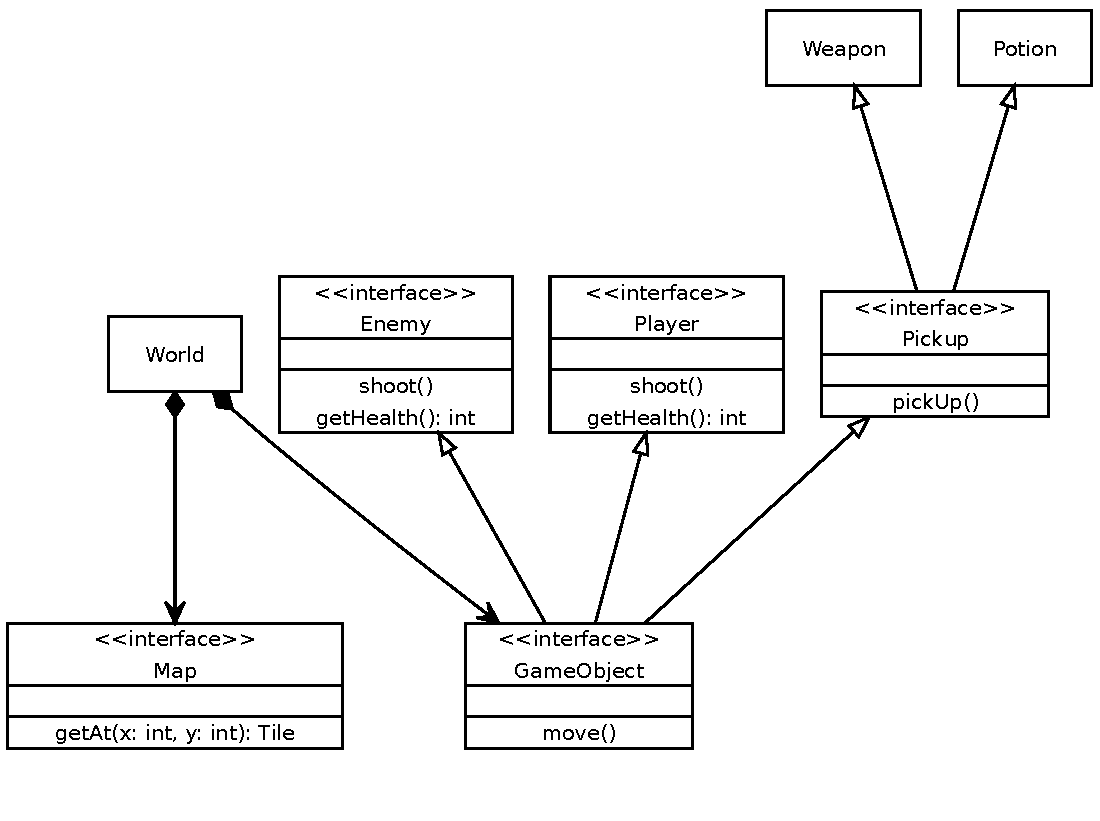
\includegraphics[width=\linewidth]{uml1}
    \end{figure}
    \chapter{Design}
    \section{Architettura}
    \par L'architettura di 'D.I.S.I's Catacombs' è stata pensata e realizzata seguendo una forma modificata e naive del pattern ECS (Entity–component–system).
    Questo pattern architetturale permette la definizione della entità di gioco, identificata solamente da un id.
    Queste enità hanno variabili che ne definiscono l'aspetto e l'interazione con il mondo di gioco.
    Il sistema itera tra le entità periodicamente durante il game loop, aggiornando le loro componenti fisiche (come posizione della entità, dimensioni
    e movimento) e grafiche (la sprite o l'animazione).
    In un pattern ECS standard più sistemi adempierebbero a compiti diversi, ma per diminuire la complessità dell'implementazione e favorire
    un codice più chiaro al gruppo si è deciso di implementare un solo sistema che esegue tutte le azioni sulle componenti delle entità e gli eventi di gioco.
    Questa genere di architettura garantisce una maggiore flessibilità nelle componenti delle entità e garantisce modifiche a runtime di quest'ultime.
    Il sistema infatti durante le iterazioni tra le entità ha la possibilità di gestirne e di eseguire la logica dei loro componenti utilizzando filtri di
    vario tipo.
    Questo permette l'integrazione di metodi di alto livello come stream, lambda, ecc\ldots.
    Gli input servono a gestire unicamente il movimento e lo sparo del Player.
    Il lato negativo dell'architettura da noi usata è che il gioco può diventare molto pesante e lento dopo un elevato numero di entità generate e visualizzate
    durante l'esecuzione.
    \section{Design dettagliato}
    \subsection{Chelli}
    \par Questa parte si concentrerà sugli aspetti relativi alla mappa di gioco.
    % UML Tile
    \par
    \begin{tikzpicture}
        \tikzstyle{every node}=[font=\scriptsize]
        \begin{class}[text width=3.5cm]{Tile}{0, 0}
            \attribute{VOID}
            \attribute{WALL}
            \attribute{FLOOR}
            \attribute{STAIRS}
            \operation{+ isWalkable(): boolean}
        \end{class}
    \end{tikzpicture}
    \par La mappa e' concettualmente una matrice di caselle, che possono essere pavimento o muro.

    \par Le caselle vengono rappresentate da un enum chiamato Tile.

    % UML TileMap
    \par
    \begin{tikzpicture}
        \tikzstyle{every node}=[font=\scriptsize]
        \begin{interface}[text width=3.5cm]{TileMap}{0, 0}
            \operation{height(): int}
            \operation{width(): int}
            \operation{at(x: int, y: int): Tile}
            \operation{canSpawnAt(x: int, y: int): boolean}
        \end{interface}
        \begin{class}[text width=3.5cm]{TileMapImpl}{6, 0}
            \implement{TileMap}
            \operation{+ getMap(): Tile[][]}
        \end{class}
    \end{tikzpicture}
    \par Per rappresentare la mappa, ho deciso di usare un interfaccia chiamata TileMap.
    Quest'interfaccia ha le poche funzioni necessarie per descrivere la rappresentazione concettuale
    descritta in precedenza.
    Anche se questa interfaccia ha una sola classe che la implementa,
    serve per astrarre l'implementazione che potrebbe cambiare col tempo
    e per lasciare spazio a nuove implementazioni possibili.
    L'implementazione attuale utilizza una matrice di Tile siccome mi sembrava la rappresentazione piu vicina al concetto di TileMap.

    % UML TileMapFactory
    \par
    \begin{tikzpicture}
        \tikzstyle{every node}=[font=\scriptsize]
        \begin{interface}[text width=3.5cm]{TileMapFactory}{0, 0}
            \operation{def(): TileMap}
            \operation{seededDef(seed: long): TileMap}
            \operation{empty(h: int, w: int): TileMap}
        \end{interface}
        \begin{class}[text width=3.5cm]{TileMapFactoryImpl}{6, 0}
            \implement{TileMapFactory}
        \end{class}
    \end{tikzpicture}
    \par Per la creazione delle TileMap ho deciso di usare una Factory,
    anche questa divisa in interfaccia e implementazione.
    La Factory fornisce metodi per avere una TileMap con parametri default,
    un metodo simile per fare la stessa cosa ma con un seed dato,
    e un metodo per una TileMap vuota, usato per testing.

    \par L'implementazione della Factory, e' divisa in diverse funzioni private
    in quanto una singola funzione risultava troppo lunga e difficile da leggere.
    Tutte le TileMap richieste dall'interfaccia della Factory, possono essere costruite con la stessa funzione internamente,
    a parte quella vuota usata per il testing.

    \subsection{Sanità}
    \par Questa parte si concentrerà sugli aspetti relativi ai vari stati che costituiscono il gioco (menu, stato di gioco, stato di fine).
    Il sistema per la creazione di questi stati è la creazione di una classe astratta State dalla quale poi verranno
    estese tutte le classi che costituiscono i diversi stati. Questa classe rappresenta lo scheletro di un qualunque
    stato ed essendo una classe astratta l’implementazione di due metodi astratti quali update e render sarà diversa da
    stato a stato in modo che la logica e la grafica di ogni stato risulti diversa.
    %UML
    \\
    \\
    \par
    \begin{tikzpicture}
        \tikzstyle{every node}=[font=\scriptsize]
        \begin{abstractclass}[text width=3.5cm]{State}{0, 0}

            \operation{+ update(delta : long)}
            \operation{+ render(g2 : Graphics2D)}
        \end{abstractclass}

        \begin{class}[text width=3.5cm]{MenuState}{-5, -5}
            \inherit{State}

            \operation{+ update(delta : long)}
            \operation{+ render(g2 : Graphics2D)}
        \end{class}

        \begin{class}[text width=3.5cm]{GameState}{0, -5}
            \inherit{State}

            \operation{+ update(delta : long)}
            \operation{+ render(g2 : Graphics2D)}
        \end{class}

        \begin{class}[text width=3.5cm]{EndGameState}{5, -5}
            \inherit{State}

            \operation{+ update(delta : long)}
            \operation{+ render(g2 : Graphics2D)}
        \end{class}

    \end{tikzpicture}
    \\
    \\
    \par Questa parte verterà sulla gestione della schermata principale e su quella di fine gioco la quale poi introdurrà nuovamente
    alla schermata di menu. Il sistema per la gestione di questi due stati è la medesima, entrambi utilizzano il pattern Strategy
    infatti è possibile modificare la grafica di queste schermate senza andare ad impattare direttamente la logica che le gestisce.
    Questa scelta è stata fatta principalmente per evitare di infrangere SRP (Single Responsibility Principle) e quindi
    di incaricare una classe sia della gestione grafica di una schermata sia della sua logica creando così una complicazione
    in un futuro cambiamento.
    %UML
    \\
    \\
    \par
    \begin{tikzpicture}
        \tikzstyle{every node}=[font=\scriptsize]
        \begin{class}[text width=3.5cm]{MenuState}{-4, -0.2}

            \operation{+ update(delta : long)}
            \operation{+ render(g2 : Graphics2D)}
        \end{class}

        \begin{interface}[text width=3.5cm]{LogicMenu}{4, 0}

            \operation{start( )}
            \operation{selectOption( )}
            \operation{getOption( )}
            \operation{isOptionStart( )}
        \end{interface}

        \aggregation{MenuState}{uses}{}{LogicMenu}

        \begin{class}[text width=3.5cm]{LogicMenuImpl}{4, -5}
            \implement{LogicMenu}

            \operation{+ start( )}
            \operation{+ selectOption( )}
            \operation{+ getOption( )}
            \operation{+ isOptionStart( )}
        \end{class}
    \end{tikzpicture}
    \\
    \\
    \par Questa parte riguarda la gestione degli asset più precisamente la creazione di strutture e il caricamento delle
    immagini all’interno di esse. Il pattern utilizzato in questo caso è Singleton permettendo che ci sia un'unica istanza
    di AssetManager accessibile globalmente senza doversi preoccupare di fornire il riferimento a chi lo richiede.
    Questa scelta è stata fatta perché il caricamento delle immagini in quelle strutture basta farla una volta sola per poi
    permetterne l’accesso a chiunque lo richieda. Lo stesso ragionamento è stato fatto per il KeyManager essendo anche esso
    di utilità a più classi evitando anche in questo caso la creazione di istanze superflue.
    %UML
    \\
    \\
    \par
        \begin{tikzpicture}
            \tikzstyle{every node}=[font=\scriptsize]
            \begin{class}[text width=6cm]{AssetManager}{-4, 0}
                \attribute{- SINGLETON\_MANAGER : AssetManager}

                \operation{- AssetManager( )}
                \operation{+ getAssetManager( )}
            \end{class}

            \begin{class}[text width=6.5cm]{KeyManager}{4, 0}
                \attribute{- SINGLETON\_KEYMANAGER : KeyManager}

                \operation{- KeyManager( )}
                \operation{+ getKeyManager( )}
            \end{class}
        \end{tikzpicture}
    \\
    \\
    \par Questa parte di codice si occupa invece della cambiamento di stato ovvero delle transizioni che portano da uno stato
    a l’altro. In questo caso è stato utilizzata una Factory di transizione per via del fatto che la forma delle transizioni
    è la medesima le uniche differenze riguardano gli stati di partenza e di arrivo e il messaggio che il giocatore vedrà.
    In questo non utilizzando una Factory avrei avuto tre classi in cui quasi tutto il codice veniva ripetuto e solo poche
    parti sarebbero cambiate e così facendo avrei violato una regola base generale di buona programmazione ovvero
    DRY (Don’t Repeat Yourself).
    %UML
    \\
    \\
    \par
    \begin{tikzpicture}
        \tikzstyle{every node}=[font=\scriptsize]

        \begin{abstractclass}[text width=3.5cm]{State}{-4, 0}

            \operation{+ update(delta : long)}
            \operation{+ render(g2 : Graphics2D)}
        \end{abstractclass}

        \begin{interface}[text width=3.5cm]{TransitionFactory}{4, 0}

            \operation{transState(message : String, game : DungeonGame, state : State)}
        \end{interface}

        \begin{class}[text width=3.5cm]{TransitionFactoryImpl}{4, -5}
            \implement{TransitionFactory}

            \operation{- generalTrans(message : String, game : DungeonGame, state : State)}
            \operation{+ transState(message : String, game : DungeonGame, state : State)}
        \end{class}

        \association{TransitionFactory}{creates}{}{State}{}{}
    \end{tikzpicture}
    \\
    \\
    \subsection{Monti}
    \par In questa sezione ci si concentrerà sugli aspetti riguardanti gli oggetti e le entità del gioco e della loro generazione.
    \par Dovendo creare oggetti con elementi in comune ho deciso di utilizzare un Template Method che ha come template la classe astratta GameObject
    Questa ha lo scopo di identificare un oggetto di gioco caratterizzato da poche elementali caratteristiche come la posizione nella mappa, la velocità e
    le dimensioni che esso ha.
    Inoltre viene specificato il metodo update nel quale gli oggetti di gioco aggiorneranno i loro stati, si muoveranno e/o spareranno o compieranno
    altre azioni.
    Il template viene poi esteso alle classi Entity, Weapon, SimplePotion e Projectile.
    \\
    \par
    \begin{tikzpicture}
        \tikzstyle{every node}=[font=\scriptsize]
        \begin {abstractclass}[text width=10cm]{GameObject}{0, -8}
            \attribute {\#posX: int}
            \attribute {\#posY: int}
            \operation {\#kind: GameObjectType}
            \attribute {\#speedX: int}
            \attribute {\#speedY: int}
            \attribute {\#hitBox: CollisionBox}
            \attribute {\#team: Team}
            \operation {+update(delta: long, others: List<GameObject>): List<GameObject>}
        \end {abstractclass}

        \begin {abstractclass}[text width=5cm]{Entity}{-5, 0}
            \inherit {GameObject}
            \attribute {\#face: Direction}
            \attribute {\#hp: int}
            \operation {\#kind: GameObjectType}
            \attribute {\#width: int}
            \attribute {\#height: int}
            \attribute {\#size: int}
            \attribute {\#tileMap: TileMap}
            \operation {\#move: void}
        \end {abstractclass}

        \begin {abstractclass}[text width=5cm]{Weapon}{+5, 0}
            \inherit {GameObject}
            \attribute {\#strength: int}
            \attribute {\#ps: int}
            \operation {\#fireRate: long}
            \attribute {\#canFire: boolean}
            \attribute {\#fireDelay: long}
            \attribute {\#fireDelayCount: long}
            \operation {+fire(psx: int, psy: int): void}
        \end {abstractclass}

    \end{tikzpicture}
    \\
    \begin{center}
        In figura è rappresentato lo schema del Template Method del GameObject
    \end{center}
    \par Sempre con in mente il Template Method ho deciso di rendere astratte le classi Entity e Weapon, essendo entrambe una generalizzazione di quelli
    che sono rispettivamente i diversi personaggi (come il Player e i nemici) e le diverse armi presenti nel gioco.
    In particolare Entity è una classe astratta che rappresenta l'insieme degli oggetti definiti Living ("vivi"), cioè che si muovono, hanno una salute
    e compiono azioni tramite input o in modo autonomo (come muoversi, sparare o lasciare oggetti).
    Nel gioco sono attualmente implementate solo alcune entità basilari, ovvero il Player e tre nemici: Bat, Slime e Boss. Il metodo template però permette
    facilmente di aggiungere in futuro altre entità (p.e.: nuovi nemici, NPC, ecc.).
    Allo stesso tempo anche la classe astratta Weapon definisce l'insieme delle armi utilizzabili. Come Entity ci sono per ora solamente due tipi di Weapon
    chiamate Gun e Rifle ma è possibile aggiungerne altre facilmente.
    \\
    \par
    \begin{tikzpicture}
        \tikzstyle{every node}=[font=\scriptsize]

        \begin {abstractclass}[text width=10cm]{Entity}{-10, -10}
            \attribute {\#face: Direction}
            \attribute {\#hp: int}
            \operation {\#kind: GameObjectType}
            \attribute {\#width: int}
            \attribute {\#height: int}
            \attribute {\#size: int}
            \attribute {\#tileMap: TileMap}
            \operation {+update(delta: long, others: List<GameObject>): List<GameObject>}
            \operation {\#move: void}
        \end {abstractclass}

        \begin {class}[text width=6cm]{Bat}{-15, 0}
            \inherit {Entity}
            \operation {+setShootingDirection(e: GameObject): void}
            \operation {-changeDirection: void}
        \end {class}

        \begin {class}[text width=6cm]{Boss}{-10, -5}
            \inherit {Entity}
            \operation {+setShootingDirection(e: GameObject): void}
            \operation {-changeDirection: void}
        \end {class}

        \begin {class}[text width=6cm]{Slime}{-7, 0}
            \inherit {Entity}
            \operation {+setCharacterToFollow(e: GameObject): void}
            \operation {-follow(): void}
        \end {class}

    \end{tikzpicture}
    \\
    \begin{center}
        In figura è rappresentato lo schema del Template Method della Entity
    \end{center}
    \par
    \begin{tikzpicture}
        \tikzstyle{every node}=[font=\scriptsize]

        \begin {abstractclass}[text width=10cm]{Weapon}{-5, -5}
            \attribute {\#strength: int}
            \attribute {\#ps: int}
            \operation {\#fireRate: long}
            \attribute {\#canFire: boolean}
            \attribute {\#fireDelay: long}
            \attribute {\#fireDelayCount: long}
            \operation {+update(delta: long, others: List<GameObject>): List<GameObject>}
            \operation {+fire(psx: int, psy: int): void}
        \end {abstractclass}

        \begin {class}[text width=6cm]{Gun}{-10, 0}
            \inherit {Weapon}
            \operation {+getStrength(): int}
            \operation {+getFireRate(): int}
            \operation {+getProjectileSpeed(): int}
        \end {class}

        \begin {class}[text width=6cm]{Rifle}{0, 0}
            \inherit {Weapon}
            \operation {+getStrength(): int}
            \operation {+getFireRate(): int}
            \operation {+getProjectileSpeed(): int}
        \end {class}
    \end{tikzpicture}
    \\
    \begin{center}
        In figura è rappresentato lo schema del Template Method della Weapon
    \end{center}
    \par Per la generazione degli oggetti di gioco ho deciso di distinguere la generazione delle entità da quella degli oggetti.
    La decisione di implementare due factory invece che una deriva da due fattori:
    \begin{itemize}
        \item Chiarezza dei nomi delle factory in relazione agli elementi creati
        \item Crezione di sole Entity per facilitare l'utilizzo
    \end{itemize}
    Cosi facendo la MobFactory gestisce la creazione di tutte le Entity sulla mappa, mentre la ObjectFactory gestisce i GameObject.
    Le factory forniscono metodi semplici per lo spawn, che avviene solamente solamente se la posizione selezionata (o generata randomicamente) è accessibile
    nella mappa.
    \\
    \par
    \begin{tikzpicture}
        \tikzstyle{every node}=[font=\scriptsize]

        \begin {interface}[text width=8.5cm]{ObjectFactory}{0, 0}
            \operation {spawnAt(x: int, y: int, f: SingleObject<GameObject>): List<GameObject>}
            \operation {spawnSome(n: int, f: SingleObject<GameObject>): List<GameObject>}
        \end {interface}

        \begin {class}[text width=8.5cm]{ObjectFactoryImpl}{0, -5}
            \implement{ObjectFactory}
            \operation {+setNewTileMap(tileMap: TileMap): void}
        \end {class}

    \end{tikzpicture}
    \\
    \\
    \begin{center}
        In figura è rappresentato lo schema del Factory Method della ObjectFactory
    \end{center}
    \par
    \begin{tikzpicture}
        \tikzstyle{every node}=[font=\scriptsize]

        \begin {interface}[text width=8.5cm]{MobFactory}{0, 0}
            \operation {spawnAt(x: int, y: int, f: SingleObject<GameObject>): List<Entity>}
            \operation {spawnSome(n: int, f: SingleObject<GameObject>): List<Entity>}
            \operation {spawnRandom(): List<Entity>}
            \operation {spawnNear(range: int, e: GameObject, f: SingleObject<GameObject>): List<Entity>}
        \end {interface}

        \begin {class}[text width=8.5cm]{MobFactoryImpl}{0, -5}
            \implement{MobFactory}
            \operation {+setNewTileMap(tileMap: TileMap): void}
        \end {class}

    \end{tikzpicture}
    \\
    \\
    \begin{center}
        In figura è rappresentato lo schema del Factory Method della MobFactory
    \end{center}
    \subsection{Tampieri}
    \par Durante lo sviluppo ho notato la necessità di utilizzare due diversi design pattern.
    \subsubsection{\texttt{ImageTransformer} Abstract Factory}
    \par
    \begin{tikzpicture}
        \tikzstyle{every node}=[font=\scriptsize]
        \begin{interface}[text width=4cm]{ImageTransformerFactory}{0, 0}
            \operation{ + rotate(degrees: double): ImageTransformer}
            \operation{ + scale(scalingFactor: double): ImageTransformer}
            \operation{ + flip(flipX: boolean, flipY: boolean): ImageTransformer}
        \end{interface}
        \begin{class}[text width=4.5cm]{ImageTransformerFactoryImpl}{6, 0}
            \implement{ImageTransformerFactory}
            \operation{ + rotate(degrees: double): ImageTransformer}
            \operation{ + scale(scalingFactor: double): ImageTransformer}
            \operation{ + flip(flipX: boolean, flipY: boolean): ImageTransformer}
        \end{class}
    \end{tikzpicture}
    \par Questa Abstract Factory si è rivelata necessaria perché venivano effettuate diverse operazioni di trasformazione di
    immagini in più parti del codice.
    \par Per favorire il riuso e ridurre la complessità ho deciso di creare un'interfaccia \texttt{ImageTransformer}, che si occupa di applicare una certa trasformazione ad una immagine.
    \par Una factory di \texttt{ImageTransform} ritorna la trasformazione richiesta, che può essere applicata a più immagini.
    \par Un vantaggio di questo pattern, che per ora non viene sfruttato, è fornire diversi algoritmi di trasformazione
    nel caso quelli implementati non siano sufficientemente efficienti.
    \subsubsection{AssetManager Proxy}
    \begin{tikzpicture}
        \tikzstyle{every node}=[font=\scriptsize]
        \begin{class}[text width=12cm]{AssetManagerProxy}{6, 0}
            \attribute{- MAP\_CACHE: Map<Tile, BufferedImage>}
            \attribute{- ANIMATIONS\_CACHE: Map<Triple<Entity, Action, Direction>, Pair<Animation, Long>>}
            \attribute{- STATIC\_ASSETS\_CACHE: Map<StaticEntityKind, BufferedImage> }

            \operation{- AssetManagerProxy()}
            \operation{+ getFrames(entity: Entity, action: Action, direction: Direction): Animation}
            \operation{+ getSprite(entity: GameObject): BufferedImage}
            \operation{+ getTileSprite(tile: Tile): Optional<BufferedImage>}
        \end{class}
    \end{tikzpicture}
    \par Conscio del fatto che non si tratti di un Proxy in senso lato, ho deciso di adattare il pattern al nostro caso
    d'uso per consentire un migliore utilizzo dell'\texttt{AssetManager}, che prende in input stringhe, effettuando una
    validazione dei parametri di input e trasformandoli in stringhe, riducendo così le fonti d'errore.
    \par Inoltre, tramite questa classe, effettuo il caching delle immagini, cosa che, soprattutto nel caso di immagini
    cui viene appplicata una trasformazione, riduce il tempo di rendering.
    \chapter{Sviluppo}
    \section{Testing automatizzato}
    \par Il gruppo ha realizzato testing automatizzato tramite una suite JUnit 5 di diversi componenti chiave
    per verificare che aderissero alle specifiche.
    \par In particolare:
    \begin{itemize}
        \item Per le componenti che gestiscono I/O (\texttt{AssetManagerTest}, \texttt{UIUtilsTest} e \texttt{GameSheetTest}) viene verificato che l'accesso a risorse inesistenti venga gestito correttamente
        \item Per le componenti che gestiscono la logica del gioco (\texttt{CharactersTest} e \texttt{EquipmentTest}) viene controllato che le operazioni sugli oggetti causino i risultati atteso, come ad esempio la diminuzione del punteggio salute dopo essere stati colpiti da un proiettile
        \item Per la generazione casuale della mappa (\texttt{MapTest}) viene controllato che le mappe generate rispondano a certe caratteristiche e che la loro generazione non generi eccezioni
        \item Per lo spawn delle entità (\texttt{MobFactoryTest}) viene testata la corretta generazione delle stesse
        \item Per la gestione della logica di visualizzazione e di interazione (\texttt{CameraTest}, \texttt{CollisionBoxTest} e \texttt{HIDTests}) viene controllato che la logica della visualizzazione sa corretta nel primo caso, e che vengano gestiti correttamente gli eventi nei restanti due
    \end{itemize}
    \par Si è inoltre deciso di avere una test coverage minima obbligatoria, fissata al 50\%, e di testare tramite una pipeline (utilizzando Github Actions) per evitare di introdurre regressioni nel branch principale.
    \section{Metodologia di lavoro}
    \subsection{Chelli}
    I file che ho sviluppato interamente io o quasi sono:
    \begin{itemize}
        \item Tile
        \item TileMap
        \item TileMapImpl
        \item TileMapFactory
        \item TileMapFactoryImpl
        \item Projectile
    \end{itemize}
    Le dipendenze della TileMap con il resto del progetto e' minima, e la progettazione iniziale e' stata abbastanza ben costituita
    in quanto ho dovuto aggiungere funzioni solo una volta su richiesta degli altri membri,
    e questa modifica e' stata molto semplice e di poche righe.
    Oltre ha questo ho contribuito in diverse classi per aggiungere feature o fare refactor di parti problematiche.
    Abbiamo tutti usato git creando nuovi branch per ogni cambiamento richiesto,
    facendo uso di task automtizzati su github per il controllo di errori e stile del codice,
    e richiedendo review ai collaboratori per ogni pull request al master.

    \subsection{Sanità}
    \par In questa parte esporrò il mio contributo per il progetto relativo alle interfacce grafiche al caricamento di risorse grafiche
    e testuali , alla gestione degli asset e delle animazioni del gioco , alla struttura del loop principale attraverso il quale si
    sviluppa il gioco e alla interazione con dispositivi esterni quali mouse e tastiera.
    \par La parte di cui mi sono maggiormente e occupato la GUI del gioco nello specifico la gestione degli stati attraverso i quali
    il gioco si sviluppa partendo dalla creazione di un generico stato \texttt{State} dal quale si estendono poi altri stati quali:
    \texttt{MenuState} , \texttt{GameState} e \texttt{EndGameState}.
    \par Un’altra parte di cui mi sono occupato riguarda le transizioni ovvero il cambiamento da uno stato a l’altro attraverso la creazione
    , per mezzo di  \texttt{TransitionFactory} , di un interfaccia che fa da ponte tra due stati. La gestione di degli stati e dei loro
    cambiamenti è affidata ad un'altra classe DungeonGame anche questa implementata da me. Questa classe si occupa di controllare
    in quale stato si trova il gioco e in quale stato dovrà trovarsi se il player muore o se finisce il gioco, in poche parole la
    classe che gestisce la visualizzazione il funzionamento e il susseguirsi degli stati di gioco. Inoltre fornisce informazioni
    riguardanti la finestra principale del gioco creata dalla classe \texttt{MainWindow} di mia implementazione anche se la totalità delle
    informazioni riguardanti la finestra è disponibile a chi  ne facesse uso nella mia classe \texttt{GameConfiguration}.
    \par Il \texttt{DungeonGame} estende la classe \texttt{Game} che contiene i metodi necessari all’inizializzazione della finestra di gioco,
    il render degli aspetti di base ma soprattutto si occupa del loop principale del gioco.
    \par Un’altra classe di del mio codice è la gestione degli input di dispositivi esterni quale la tastiera \texttt{KeyManager} che
    gestisce i vari input da tastiera.
    \par Una altra parte di mia responsabilità è il caricamento di risorse come si può vedere dal package \texttt{catacombs/ui/utils (FontUtils, ImageLoader e ImageRotator)}
    e dall’\texttt{AssetManager} che fa uso di un’altra classe, \texttt{GameSheet} che si occupa di ritagliare le immagini in immagini più piccole
    in modo da separare i singoli frame di movimento dei personaggi. Tali frames verranno poi utilizzati dalla classe \texttt{Animation} che
    provvede a sequenziarli in modo da farli risultare parte di un unico fluido movimento.
    \par Usufruendo delle funzinalità di branching che Git offre è stato facile rimanere aggiornato sugli sviluppi del progetto anche non
    relativi alle mie implenatazioni. la metodologia utilizzata cosnisteva nell' utilizzo di un master principale da aggiornale solo con
    il codice ultimato e più volte controllato da me e dai miei compagni. Ogni parte di codice da me realizzata si sviluppava all'interno di branch
    in modo da non sporcare il codice definitivo contenuto nel master. solo dopo aver ultimato ogni modifica ed aver ottenuto l'approvazione dei miei colleghi
    il branch veniva mergiato con il master.
    La suddivisione dei lavori precedentemente stabilita veniva rispecchiata nella spartizione degli issue ovvero degli obbiettivi parziali da risolvere che uniti
    andavano a comporre una parte sostanziosa di codice.
    \subsection{Monti}
    \par Mi sono interessato per la quasi totalità ai GameObject e alle classi che lo estendono ad esclusione del Player, SimplePotions e Projectiles.
    In particolare mi sono occupato dell'analisi e della creazione di GameObject, di Entity, di Weapon e del package model.gen contenenti le Factory MobFactory
    e ObjectFactory.
    Sviluppo dei nemici Bat, Slime e Boss, della Weapon e classi derivate Gun e Rifle.
    Refactoring di alcune classi e metodi. Implementazione di piccole feature in classi altrui.
    Per ogni cambiamento o feature è stato creato un branch ed è stata richiesta la review per la pull request al master.
    Inoltre ho aggiunto qualche sprite al gioco.
    \subsection{Tampieri}
    \par Ho realizzato le seguenti classi:
    \begin{itemize}
        \item \texttt{eu.eutampieri.catacombs.model.Action}
        \item \texttt{eu.eutampieri.catacombs.model.Direction}
        \item \texttt{eu.eutampieri.catacombs.model.HealthModifier}
        \item \texttt{eu.eutampieri.catacombs.model.LivingCharacter}
        \item \texttt{eu.eutampieri.catacombs.model.Player}, con contributi minimi di Monti
        \item \texttt{eu.eutampieri.catacombs.model.SimplePotion}
        \item \texttt{eu.eutampieri.catacombs.ui.gamefx.Animatable}
        \item \texttt{eu.eutampieri.catacombs.ui.gamefx.AssetManagerProxy}
        \item \texttt{eu.eutampieri.catacombs.ui.utils.ImageTransformer}
        \item \texttt{eu.eutampieri.catacombs.ui.ImageTransformerFactory}
        \item \texttt{eu.eutampieri.catacombs.ui.ImageTransformerFactoryImpl}
        \item \texttt{eu.eutampieri.catacombs.ui.World}
    \end{itemize}
    \par Ho inoltre realizzato alcune bugfixes nel codice da me usato, in particolare in \texttt{eu.eutampieri.catacombs.ui.Game}, \texttt{eu.eutampieri.catacombs.model.GameObject} e \texttt{eu.eutampieri.catacombs.model.Entity}.
    \par Tranne che per le modifiche di classi o interfacce comuni, non ho avuto particolari problemi dovuti allo sviluppo in parallelo,
    anche grazie all'utilizzo di \texttt{git}, di cui ho sfruttato il branching e il cherry pick.
    \section{Note di sviluppo}
    \subsection{Chelli}
    \begin{itemize}
        \item Uso di stream per facilitarmi nell'algoritmo di generazione della mappa
        \item Uso di lambda expression insieme agli stream
        \item Abbiamo usato gradle
        \item L'algoritmo usato per generare la mappa, essendo molto specifico non e' fornito da librerie esterne
    \end{itemize}
    \subsection{Sanità}
    \begin{itemize}
        \item Uso di Optional per la gestione degli eventuali file non trovati
        \item Uso di basilari lambda expressions nei test automatizzati
    \end{itemize}
    \subsection{Monti}
    \begin{itemize}
        \item Streams
        \item Lambda expressions
        \item Generici nelle factory
        \item Apache commons per l'utilizzo dei pair
    \end{itemize}
    \subsection{Tampieri}
    \par Ho utilizzato le seguenti funzionalità avanzate del linguaggio:
    \begin{itemize}
        \item Generici bounded, utilizzati per estendere il \texttt{SingleObject} realizzato da Giacomo Monti
        \item Uso di lambda expression in \texttt{AssetManagerProxy} e \texttt{ImageTransformerFactoryImpl}
        \item Uso di \texttt{Stream} in \texttt{AssetManagerProxy}
        \item Utilizzato (seppur marginalmente) Apache Commons Lang: nello specifico \texttt{Pair} e \texttt{Triple}
        \item Configurato Gradle, partendo dall'esempio fornitoci e integrandolo con la static code analysis
    \end{itemize}
    \par Ho utilizzato i seguenti snippet di codice:
    \begin{itemize}
        \item How to scale a \texttt{BufferedImage}\cite{so:BufferedImageScaling},\\\texttt{src/main/java/eu/eutampieri/catacombs/ui/utils/ImageTransformerFactoryImpl.java}, linee 23-29.
    \end{itemize}
    \chapter{Commenti finali}
    \section{Autovalutazione e lavori futuri}
    \subsection{Chelli}
    Il mio lavoro si concentrava su una parte chiave nel progetto anche se non centrale,\\
    per questo mi e' stato facile lavorare sul mio progetto in modo indipendente,\\
    riportando un risultato piu che soddisfacente senza particolari problemi.\\
    Anche se il progetto potrebbe essere portato avanti, non e' nelle mie intenzioni farlo,\\
    visto che come gioco non porta avanti niente di nuovo o interessante.\\
    \subsection{Sanità}
    \par Questo progetto è stato veramente impegnativo ed è stato in grado di far risaltare le mie lacune riguardo sopratutto l'utilizzo di \texttt{git} che come
    primo approccio è stato abbastanza brusco, mi sono ritrovato catapultato in una gestione condivisa dei file che non avevo mai usato.
    \par Per quanto riguarda l'implementazione dei metodi e delle interfacce la difficoltà non è stata esagerata in quanto è bastato trovare una soluzione
    architetturale decente prima di scrivere righe di codice.
    \subsection{Monti}
    Le difficoltà principali le ho riscontrate durante l'analisi del modello, essendo la prima esperienza di game design.
    Le debolezze del gioco sono la poca varietà di armi e nemici e la grafica non troppo moderna, ma grazie al lavoro per ora svolto
    aggiungere nemici e armi risulterà molto semplice se mai si vorrà.
    \subsection{Tampieri}
    \par Personalmente ritengo che la parte di progettazione delle mie classi sia nel complesso positiva, perché
    ho strutturato il codice in modo abbastanza flessibile, soprattutto grazie all'uso di interfacce per astrarre
    i comportamenti dalle implementazioni.
    \par Inoltre, il codice è strutturato in modo da rendere abbastanza semplice creare un gioco multiplayer, cosa
    che potrebbe essere realizzata in una versione successiva.
    \par Ciononostante, ci sono alcune parti ampiamente migliorabili, come il collegamento degli asset realizzato
    nell'\texttt{AssetManagerProxy}, che renderà complessa l'aggiunta di nuove entità in futuro.
    \section{Difficoltà incontrate e commenti per i docenti}
    \subsection{Tampieri}
    \par Durante lo svolgimento del progetto mi è stato abbastanza difficile coordinarmi con il resto del gruppo per
    realizzare le parti di mia responsabilità.
    \par Ritengo che questo sia dovuto al non aver raggiunto un livello di dettaglio in fase di progettazione a me
    sufficiente per capire effettivamente la struttura del progetto.
    \par Il deficit sottolineato sopra ha portato ad alcune discussioni sul design delle classi, soprattutto su come
    mantenerle retrocompatibili ma adeguandole ad esigenze non emerse in fase di progettazione.
    \appendix
    \chapter{Guida utente}
    \par Il gioco comincerà con una schermata di menu che permette di cambiare l'opzione che si desidera scegliere attraverso l'uso
    dei tasti direzionali o  WASD, per selezionare la chiusura della finestra o l'avvio del gioco.
    \par Una volta che l'indicatore di selezione si sarà spostato sull'opzione desiderata è sufficiente premere il tasto invio per confermarla.
    \par Iniziata la partita, il personaggio si potrà spostare la mappa utilizzando i tasti indicati in precedenza.
    \par Il giocatore potrà sparare ai nemici per eliminarli usando il tasto spazio, sia tenendolo premuto che premendolo ripetutamente,
    e per poter mirare al nemico basterà rivolgere il corpo del giocatore nella direzione desiderata (e.g se un nemico si trova alla
    proria destra, l'utente dovrà premere D e poi premere la barra dello spazio).
    \par Nella mappa sono presenti alcuni oggetti utili, che possono essere raccolti camminandoci sopra.
    \par Nello specifico, sono presenti delle pozioni (rappresentate da un'ampolla) per aumentare la propria vita e delle armi. Queste ultime possono essere:
    \begin{itemize}
        \item Una pistola, che è l'arma con cui il giocatore inizia il gioco.
        \item Un fucile automatico che, rispetto alla pistola, permette di sparare più frequentemente.
    \end{itemize}
    \par Dopo aver ucciso un nemico, è possibile che questo lasci cadere un'arma o una pozione.
    \par Il gioco termina dopo aver ucciso il boss e tutti i nemici.
    \chapter{Esercitazioni di laboratorio}
    \section{Tampieri}
    \begin{itemize}
        \item Laboratorio 5: https://virtuale.unibo.it/mod/forum/discuss.php?d=62684\#p101017
        \item Laboratorio 6: https://virtuale.unibo.it/mod/forum/discuss.php?d=62579\#p100872
        \item Laboratorio 7: https://virtuale.unibo.it/mod/forum/discuss.php?d=62582\#p100877
        \item Laboratorio 8: https://virtuale.unibo.it/mod/forum/discuss.php?d=63632
    \end{itemize}
    \printbibliography[heading=bibintoc]
\end{document}
